\chapter{Rezultati i analiza}
\label{ch:rezultati-i-analiza}
Ovo poglavlje opisuje način i količinu skupljenih podataka za učenje neuronske mreže te dobivene rezultate. Napravljena
je analiza pogrešno klasificiranih znamenki kako bi se dobili uvidi u ograničenja odabranog pristupa te potencijalna
poboljšanja koja je moguće provesti.


\section{Skupljeni skup podataka}
\label{sec:skupljeni-skup-podataka}
Za potrebe raspoznavanja znamenaka \emph{JMBAG}-a bilo je potrebno istrenirani neuronsku mrežu koristeći dovoljno velik
i raznolik skup podataka za učenje deseteroznamenkastih brojeva. Većina podataka za učenje skupljena je koristeći
predložak dostupan u dodatku\ \ref{ch:predlozak-za-skupljanje-podataka-za-treniranje} dok je manji dio podataka koji je
skupljen na početku pisan na čistom papiru bez korištenja predloška. Ukupno je skupljeno 1523 deseteroznamenkastih
brojeva od 33 različitih osoba. Brojevi skupljeni od prve tri osobe pisani su na čistom papiru bez predloška te je
takvih brojeva ukupno 397. Brojevi koji su pisani bez predloška više variraju u veličini i poziciji od brojeva koji su
skupljeni koristeći predložak, međutim nije bilo potrebno raditi nikakvo dodatno ručno pretprocesiranje radi toga.
Dodatno procesiranje tih brojeva bilo je potrebno u rijetkim slučajevima u kojima zbog osvjetljenja slike brojevi nisu
bili dovoljno odvojivi od pozadine. Razlog tome je činjenica da tih 397 brojeva nije bilo skenirano kao ostatak
prikupljenog skupa brojeva nego su slikani mobilnim uređajem. Ipak, za većinu njih točnost raspoznavanja je usporediva
sa skeniranim brojevima. S druge strane, kod brojeva skupljenih koristeći predložak nije bilo potrebno nikakvo
pretprocesiranje. Brojevi su nakon skeniranja ručno izrezani iz svakog predloška i labele su im dodijeljene koristeći
prvih deset znakova imena datoteke u koju je broj spremljen. Prilikom ovog postupka neki brojevi bili su izbačeni jer su
previše presijecali linije pravokutnika predloška unutar kojih su morali biti upisani. Ovakvih brojeva bilo je samo
nekoliko, pa zbog toga skup skupljenih podataka nije značajno smanjen. Svih 1523 skupljenih brojeva nasumično je
podijeljeno u skup za treniranje koji sadrži ukupno 1141 broj i skup za testiranje koji sadrži preostala 382 broja
tako da je približna podjela $75\%$ u skupu za treniranje i $25\%$ u skupu za testiranje. Pri tome se podjela radila za
svaki od 33 skupljenih rukopisa zasebno kako bi se u oba skupa osigurala jednolika raznolikost rukopisa.


\section{Strukture treniranih neuronskih mreža i ostvareni rezultati}
\label{sec:strukture-treniranih-neuronskih-mreza-i-ostvareni-rezultati}
Bitan faktor koji utječe na točnost raspoznavanja je struktura naučene neuronske mreže. Ako neuronska mreža ima premalen
broj i dimenzije skrivenih slojeva neće biti moguće dobiti klasifikator koji može ispravno raspoznavati svih deset
različitih znamenki neovisno o broju iteracija treniranja mreže. U tom će slučaju neuronska mreža imati premalen
kapacitet da nauči veze među značajkama koje čine razlike među pojedinim znamenkama. S druge strane, ako neuronska mreža
koja se trenira ima previše skrivenih slojeva velikih dimenzija onda može doći do pretreniranja koje uzrokuje veliku
točnost na skupu za učenje ali malu točnost na ispitnom skupu. Tada neuronska mreža ima prevelik kapacitet što
uzrokuje lošu generalizaciju mreže na podatcima koji se ne nalaze u skupu za učenje. Uzrok tome je to što zbog velikog
kapaciteta mreža može zapamtiti viđene primjere za učenje umjesto pronaći veze među značajkama preko kojih se mogu
raspoznavati pojedine znamenke. Jedan od načina na koji se ovo može izbjeći je provjera greške na ispitnom skupu
prilikom postupka učenja neuronske mreže. Kada greška na ispitnom skupu počne rasti postupak učenja treba prekinuti kako
se neuronska mreža ne bi pretrenirala. Kako bi se pronašla optimalna struktura neuronske mreže, učene su mreže sa
dimenzijama:
\begin{enumerate}
    \item $36 \times 10 \times 10$,
    \item $36 \times 20 \times 10$,
    \item $36 \times 30 \times 10$,
    \item $36 \times 10 \times 10 \times 10$,
    \item $36 \times 15 \times 15 \times 10$,
    \item $36 \times 20 \times 10 \times 10$,
    \item $36 \times 20 \times 20 \times 10$,
    \item $36 \times 15 \times 10 \times 5 \times 10$.
\end{enumerate}
Sve mreže su učene na istom skupu za učenje. Postupak učenja neuronskih mreža provodio se za svaku mrežu sve dok
prosječna greška na ispitnom skupu kroz zadnjih 1000 iteracija algoritma nije počela rasti. Kroz prvih 500 iteracija
algoritma korišten je \emph{mini-batch Backpropagation} s veličinom od 100 uzoraka za učenje te stopom učenja
$\eta = 2.5$. Kroz preostale iteracije postupka učenja korišteni su svi uzorci za učenje uz stopu učenja $\eta = 2$ i
koeficijent inercije $\alpha = 0.5$. Slika\ \ref{fig:error-chart} prikazuje iznos greške na skupu za učenje te ispitnom
skupu kroz prvih 1000 iteracija za neuronsku mrežu strukture $36 \times 10 \times 10$.
\begin{figure}[htb]
    \centering
    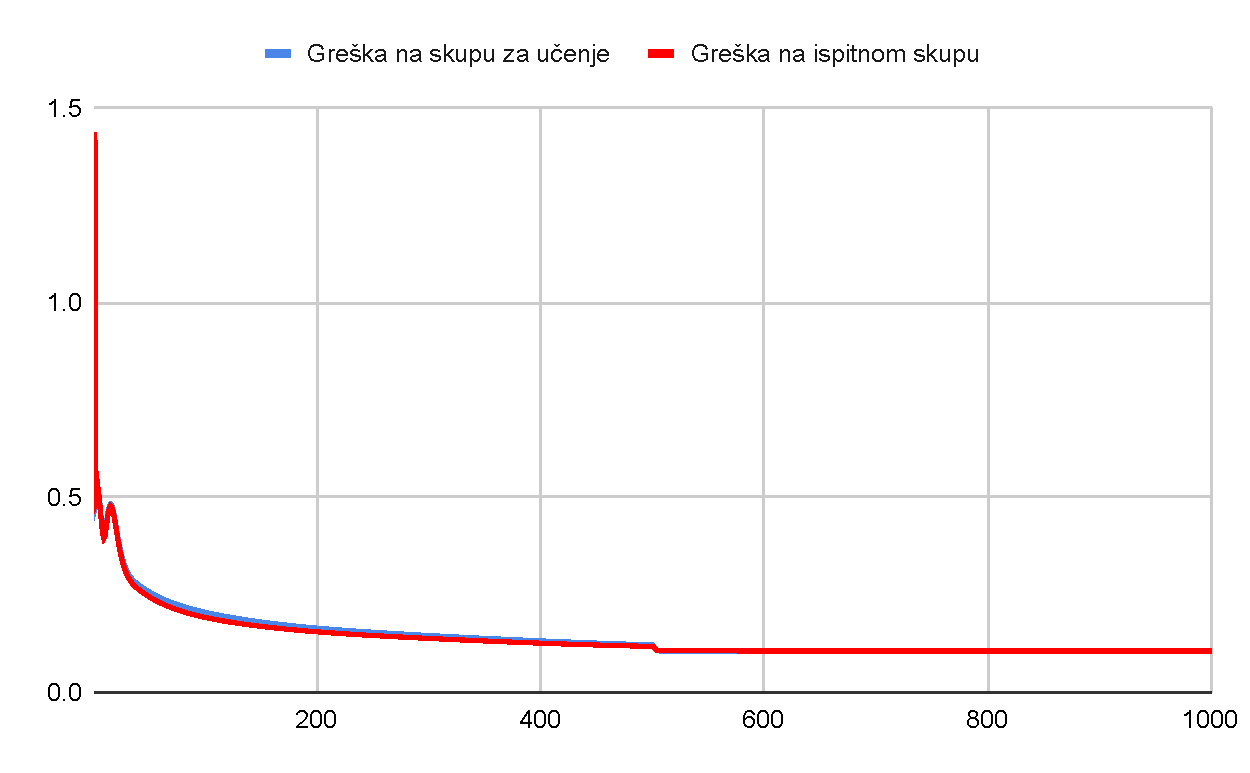
\includegraphics[width=12cm]{images/chapter5/error-chart.pdf}
    \caption{Graf vrijednosti greške na skupu za učenje i ispitnom skupu kroz prvih 1000 iteracija algoritma
    \emph{Backpropagation}.}
    \label{fig:error-chart}
\end{figure}
\newline
Tablica\ \ref{tab:nn-results} prikazuje postignute postotke ispravnih klasifikacija na skupu za učenje i na ispitnom
skupu za svaku od navedenih struktura neuronskih mreža.
\begin{table}[htb]
    \caption{Točnost različitih struktura neuronske mreže na skupu za učenje i ispitnom skupu.}
    \label{tab:nn-results}
    \scriptsize
    \centering
    \begin{tabular}{|M{4cm}|M{4cm}|M{3cm}|}
        \hline
        Struktura mreže & Točnost na skupu za učenje & Točnost na ispitnom skupu \\
        \hline
        $36 \times 10 \times 10$ & $87.57\%$ & $86.41\%$ \\
        \hline
        $36 \times 20 \times 10$ & $89.88\%$ & $88.64\%$ \\
        \hline
        $36 \times 30 \times 10$ & $91.46\%$ & $89.19\%$ \\
        \hline
        $36 \times 10 \times 10 \times 10$ & $88.58\%$ & $86.41\%$ \\
        \hline
        $36 \times 15 \times 15 \times 10$ & $91.31\%$ & $88.90\%$ \\
        \hline
        $36 \times 20 \times 10 \times 10$ & $91.64\%$ & $87.88\%$ \\
        \hline
        $36 \times 20 \times 20 \times 10$ & $91.25\%$ & $88.27\%$ \\
        \hline
        $36 \times 15 \times 10 \times 5 \times 10$ & $90.15\%$ & $86.96\%$ \\
        \hline
    \end{tabular}
\end{table}
\newline
Svih osam treniranih neuronskih mreža pokazuju prilično usporedive rezultate točnosti klasifikacije. Mreže s većim
brojem slojeva očekivano pokazuju bolje rezultate na skupu za učenje, ali ne i na ispitnom skupu. Mreža koja daje
najbolji rezultat je mreža sa strukturom $36 \times 30 \times 10$ koji pokazuje najbolju sposobnost generalizacije
raspoznavanja znamenaka. Kombiniranjem svih navedenih neuronskih mreža u jedan klasifikator koji zbraja izlaze svih
neuronskih mreža postiže se točnost raspoznavanja od $91.94\%$ na skupu za učenje te $90.08\%$ na ispitnom skupu.


\section{Analiza raspoznavanja pojedinih znamenki}
Kako naučene neuronske mreže krivo klasificiraju u prosjeku $10\%$ znamenaka, korisno je napraviti analizu raspoznavanja
svake od znamenaka kako bi se mogla napraviti potencijalna poboljšanja u postupku raspoznavanja. Stoga vrijedi
pogledati koliko ispravno naučene neuronske mreže klasificiraju svaku od pojedinih znamenki te koje znamenke čine
najveći udio netočnih klasifikacija. Time se može dobiti uvid u potencijalne sličnosti među značajkama znamenki koje
uzrokuju neispravnu klasifikaciju. Tablica\ \ref{tab:per-number-results} prikazuje postotke klasifikacija svakog od
brojeva za slučaj naučenih neuronskih mreža koje su kombinirane u jedan klasifikator.
\begin{table}[htb]
    \caption{Točnosti raspoznavanja svake od pojedinih znamenki.}
    \label{tab:per-number-results}
    \scriptsize
    \centering
    \setlength{\tabcolsep}{0.05cm}
    \begin{tabular}{|c|c|c|c|c|c|c|c|c|c|c|}
        \hline
        \diagbox{Očekivana\\znamenka}{Izlaz\\mreže} & $0$ & $1$ & $2$ & $3$ & $4$ & $5$ & $6$ & $7$ & $8$ & $9$ \\
        \hline
        $0$ & $\boldsymbol{93.56\%}$ & $0.51\%$ & $0.87\%$ & $0.36\%$ & $0.72\%$ & $0.29\%$ & $1.09\%$
        & $0.80\%$ & $0.87\%$ & $0.94\%$ \\
        \hline
        $1$ & $0.49\%$ & $\boldsymbol{96.50\%}$ & $0.57\%$ & $0.08\%$ & $0.49\%$ & $0.33\%$ & $0.16\%$
        & $0.49\%$ & $0.57\%$ & $0.33\%$ \\
        \hline
        $2$ & $0.84\%$ & $1.01\%$ & $\boldsymbol{94.28\%}$ & $0.84\%$ & $0.17\%$ & $0.42\%$ & $0.08\%$
        & $0.59\%$ & $1.26\%$ & $0.50\%$ \\
        \hline
        $3$ & $0.61\%$ & $0.61\%$ & $1.40\%$ & $\boldsymbol{89.85\%}$ & $0.52\%$ & $0.61\%$ & $0.35\%$
        & $1.40\%$ & $1.22\%$ & $3.41\%$ \\
        \hline
        $4$ & $0.74\%$ & $1.85\%$ & $0.37\%$ & $0.18\%$ & $\boldsymbol{91.59\%}$ & $1.39\%$ & $0.83\%$
        & $1.20\%$ & $0.18\%$ & $1.66\%$ \\
        \hline
        $5$ & $0.57\%$ & $0.47\%$ & $0.38\%$ & $2.08\%$ & $0.85\%$ & $\boldsymbol{90.26\%}$ & $1.61\%$
        & $0.85\%$ & $1.42\%$ & $1.51\%$ \\
        \hline
        $6$ & $1.32\%$ & $0.71\%$ & $0.91\%$ & $0.41\%$ & $1.32\%$ & $1.12\%$ & $\boldsymbol{91.88\%}$
        & $0.81\%$ & $1.52\%$ & $0.00\%$ \\
        \hline
        $7$ & $0.31\%$ & $0.63\%$ & $0.83\%$ & $0.52\%$ & $1.77\%$ & $0.73\%$ & $0.52\%$
        & $\boldsymbol{92.39\%}$ & $0.63\%$ & $1.67\%$ \\
        \hline
        $8$ & $1.98\%$ & $1.35\%$ & $0.99\%$ & $0.99\%$ & $0.45\%$ & $1.26\%$ & $0.72\%$ & $1.08\%$
        & $\boldsymbol{90.12\%}$ & $1.08\%$ \\
        \hline
        $9$ & $1.26\%$ & $1.34\%$ & $0.79\%$ & $1.73\%$ & $3.07\%$ & $1.02\%$ & $0.16\%$ & $0.79\%$
        & $1.42\%$ & $\boldsymbol{88.42\%}$ \\
        \hline
    \end{tabular}
\end{table}
\newline
Svaki redak tablice predstavlja očekivanu klasifikaciju znamenka dok stupci predstavljaju postignutu klasifikaciju
znamenke. Iz navedene tablice može se uočiti kako se najveći postotak ispravnih klasifikacija postiže za znamenku $1$
koji iznosi $96.50\%$. Razlog tome dolazi od činjenice da je broj $1$ najuža znamenka, pa će zato većina vertikalnih
značajki imati najveću moguću vrijednost, dok će skoro sve horizontalne značajke imati vrijednost oko $0.5$.
Iznenađujuće je da postotak pogrešnih klasifikacija znamenke $1$ kao znamenke $7$ značajno ne odskače od ostalih krivih
postotaka klasifikacije uzevši u obzir relativnu sličnost koso pisane znamenke $1$ i znamenke $7$. Sljedeće dvije
najbolje raspoznate znamenke su znamenka $2$ i znamenka $0$. Znamenka $2$ najčešće je krivo klasificirana kao znamenka
$8$ i znamenka $1$, dok je znamenka $0$ najčešće krivo klasificirana kao znamenka $6$ ili znamenka $9$. Dvije znamenke
za koje se postiže najgora točnost klasifikacije su znamenka $3$ s točnošću klasifikacije od $89.85\%$, te znamenka $9$
za koju se postiže najmanja točnost klasifikacije od $88.42\%$. Znamenka $3$ najčešće se pogrešno klasificira kao
znamenka $9$ što je ujedno i najveći postotak pogrešnih klasifikacija za bilo koju znamenku koji iznosi $3.41\%$.
Analizom skupljenih slika dolazi se do zaključka da je uzrok tome premalena ili previše nakošena gornja polukružnica
znamenke $3$. U tom slučaju moguće je da niti jedna od lijevih horizontalnih značajki ne pogodi rupu u polukružnici te
se zbog toga znamenka krivo klasificira. Slika\ \ref{fig:missclassified-3-as-9} prikazuje nekoliko primjera znamenke $3$
pogrešno klasificirane kao znamenka $9$.
\begin{figure}[htb]
    \centering
    \frame{
\includegraphics[width=2cm]{images/chapter5/missclassified-3-as-9-1.png}}
    \frame{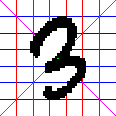
\includegraphics[width=2cm]{images/chapter5/missclassified-3-as-9-2.png}}
    \frame{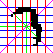
\includegraphics[width=2cm]{images/chapter5/missclassified-3-as-9-3.png}}
    \frame{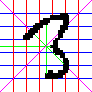
\includegraphics[width=2cm]{images/chapter5/missclassified-3-as-9-4.png}}
    \frame{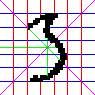
\includegraphics[width=2cm]{images/chapter5/missclassified-3-as-9-5.png}}
    \caption{Primjeri znamenke $3$ pogrešno klasificirane kao znamenka $9$.}
    \label{fig:missclassified-3-as-9}
\end{figure}
\newline
Znamenka $9$ najčešće je pogrešno klasificirana kao znamenka $4$ u $3.07\%$ slučajeva. Takva pogrešna klasifikacija se
događa u slučaju kada je znamenka $9$ pisana tako da gornja kružnica nije u potpunosti zatvorena s lijeve strane.
Ako je još uz to donji dio znamenke ravna crta, a ne kuka, čak i ljudsko oko može pogrešno klasificirati znamenku $9$
kao znamenku $4$. Nekoliko primjera znamenke $9$ pogrešno klasificirane kao znamenaka $4$ prikazano je na
slici\ \ref{fig:missclassified-9-as-4}.
\begin{figure}[htb]
    \centering
    \frame{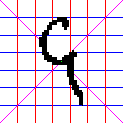
\includegraphics[width=2cm]{images/chapter5/missclassified-9-as-4-1.png}}
    \frame{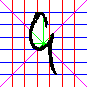
\includegraphics[width=2cm]{images/chapter5/missclassified-9-as-4-2.png}}
    \frame{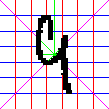
\includegraphics[width=2cm]{images/chapter5/missclassified-9-as-4-3.png}}
    \frame{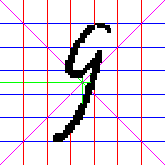
\includegraphics[width=2cm]{images/chapter5/missclassified-9-as-4-4.png}}
    \frame{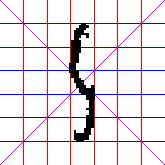
\includegraphics[width=2cm]{images/chapter5/missclassified-9-as-4-5.png}}
    \caption{Primjeri znamenke $9$ pogrešno klasificirane kao znamenka $4$.}
    \label{fig:missclassified-9-as-4}
\end{figure}
\newline
Navedene primjere pogrešnih klasifikacija ipak je moguće popraviti boljim odabirom značajki jer je segmentacija brojeva
ispravno provedena. Ako broj koji se raspoznaje nije dobro segmentiran, nikakav odabir značajki neće pružati mogućnost
raspoznavanja kroz generalizaciju te će u tim slučajevima neuronska mreža zapamtiti primjer ili ga pogrešno
klasificirati.

\section{Analiza grešaka kod segmentacije brojeva}
Kako se postupak segmentacije znamenaka provodi nalaženjem povezanih komponenti na slici, moguće je da pronađene
komponente ne odgovaraju u potpunosti pojedinačnim znamenkama. Postoje dva moguća slučaja:
\begin{enumerate}
    \item Ako se dvije ili više znamenaka međusobno dodiruju, sve će pripadati jednoj povezanoj komponenti koju je
    potrebno podijeliti na manje komponente.
    \item Ako se znamenka sastoji od više manjih povezanih komponenata, onda je potrebno te komponente povezati u jednu
    logičku grupu.
\end{enumerate}
U oba slučaja deterministički algoritam segmentacije neće raditi s  ispravnošću od $100\%$ te će neke znamenke biti
pogrešno segmentirane. Od 1523 skupljenih slika, njih 186 sadrži dvije međusobno povezane znamenke, 50 slika sadrži tri
međusobno povezane znamenke ili dvije grupe po dvije povezane znamenke dok 17 slika sadrži čak do 4 međusobno povezane
znamenke ili ekvivalentne manje povezane grupe znamenki. Ukupno 253 slike sadrži barem dvije povezane znamenke što
iznosi oko $6\%$ prikupljenih podataka. Jedan dio tih slika ipak je dovoljno dobro segmentiran koristeći algoritam
segmentiranja opisan u odjeljku\ \ref{sec:segmentacija}. Slika\ \ref{fig:segmentation-errors} prikazuje razne pogrešno
segmentirane znamenke.
\begin{figure}[htb]
    \centering
    \frame{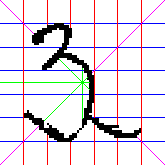
\includegraphics[width=2cm]{images/chapter5/segmentation-error-1.png}}
    \frame{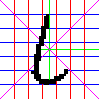
\includegraphics[width=2cm]{images/chapter5/segmentation-error-2.png}}
    \frame{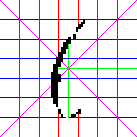
\includegraphics[width=2cm]{images/chapter5/segmentation-error-3.png}}
    \frame{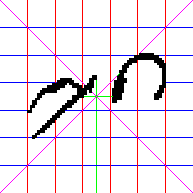
\includegraphics[width=2cm]{images/chapter5/segmentation-error-4.png}}
    \frame{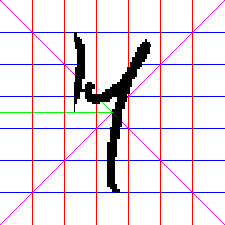
\includegraphics[width=2cm]{images/chapter5/segmentation-error-5.png}}
    \frame{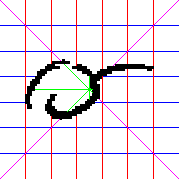
\includegraphics[width=2cm]{images/chapter5/segmentation-error-6.png}}
    \\\vspace{0.075cm}
    \frame{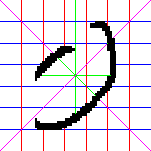
\includegraphics[width=2cm]{images/chapter5/segmentation-error-7.png}}
    \frame{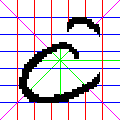
\includegraphics[width=2cm]{images/chapter5/segmentation-error-8.png}}
    \frame{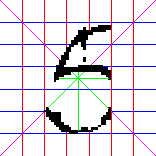
\includegraphics[width=2cm]{images/chapter5/segmentation-error-9.png}}
    \frame{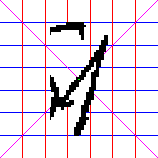
\includegraphics[width=2cm]{images/chapter5/segmentation-error-10.png}}
    \frame{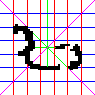
\includegraphics[width=2cm]{images/chapter5/segmentation-error-11.png}}
    \frame{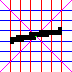
\includegraphics[width=2cm]{images/chapter5/segmentation-error-12.png}}
    \caption{Primjeri pogrešno segmentiranih znamenaka.}
    \label{fig:segmentation-errors}
\end{figure}
\newline
Najgore greške segmentacije su one koje uzrokuju pogrešnu klasifikaciju znamenaka koje su inače dobro klasificirane, ali
se zbog pomaka ne nalaze na dobrom mjestu u konačnom broju. Primjer jednog takvog slučaja prikazan je na
slici\ \ref{fig:segmentation-shift-error}.
Dolazi se do zaključka da je postupak segmentacije potrebno provesti koristeći neki drugi algoritam koji može sam
naučiti kako segmentirati brojeve. U tom slučaju potrebno je na skupljenom skupu podataka ručno označiti svaku znamenku
kako bi takav algoritam imao ulazne primjere za učenje. Kod takvog postupka označavanja moguće je koristiti
implementirani deterministički algoritam za segmentaciju jer će on dobro raditi na većini skupljenih slika. Tada je
potrebno samo podesiti oznake u neispravnim slučajevima što može značajno smanjiti vrijeme ručnog označavanja slika.
\begin{figure}[htb]
    \centering
    
\includegraphics[width=12cm]{images/chapter5/segmentation-shift-all.png}
    \\\vspace{0.075cm}
    \frame{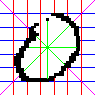
\includegraphics[width=1cm]{images/chapter5/segmentation-shift-1.png}}
    \frame{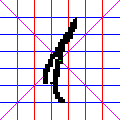
\includegraphics[width=1cm]{images/chapter5/segmentation-shift-2.png}}
    \frame{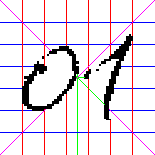
\includegraphics[width=1cm]{images/chapter5/segmentation-shift-3.png}}
    \frame{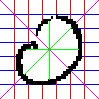
\includegraphics[width=1cm]{images/chapter5/segmentation-shift-4.png}}
    \frame{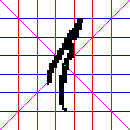
\includegraphics[width=1cm]{images/chapter5/segmentation-shift-5.png}}
    \frame{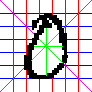
\includegraphics[width=1cm]{images/chapter5/segmentation-shift-6.png}}
    \frame{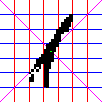
\includegraphics[width=1cm]{images/chapter5/segmentation-shift-7.png}}
    \frame{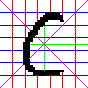
\includegraphics[width=1cm]{images/chapter5/segmentation-shift-8.png}}
    \frame{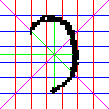
\includegraphics[width=1cm]{images/chapter5/segmentation-shift-9.png}}
    \frame{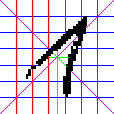
\includegraphics[width=1cm]{images/chapter5/segmentation-shift-10.png}}
    \caption{Primjer pogrešne segmentacije koja uzrokuje pomak znamenaka.}
    \label{fig:segmentation-shift-error}
\end{figure}
